\documentclass{article}

\title{Chapter 3: Vectors}
\author{Rylan Polster}

\usepackage[parfill]{parskip}
\usepackage{multirow}
\usepackage{amsmath,amssymb,amsthm}
\usepackage{bm}
\usepackage{textcomp,gensymb}
\usepackage{siunitx}
\usepackage{graphicx,float,caption}
\graphicspath{ {images/} }
\captionsetup{width=\linewidth}
\usepackage[margin=1.0in]{geometry}

\begin{document}
    \maketitle
    
    \section*{General}

        \paragraph{Quantities}
        \begin{align}
            \vec{r} &= \text{resultant vector} \nonumber\\
            |\vec{a}| &= \text{magnitude of vector $\vec{a}$} \nonumber\\
            \vec{a} \cdot \vec{b} &= \text{dot product of vectors $\vec{a}$ and $\vec{b}$} \nonumber\\
            \vec{a} \times \vec{b} &= \text{cross product of vectors $\vec{a}$ and $\vec{b}$} \nonumber\\
            \theta &= \text{angle between a vector and the $+x$ axis} \nonumber\\
            \phi &= \text{smallest angle between two vectors} \nonumber
        \end{align}

    \section{Vectors and Their Components}

        \paragraph{Commutative Law For Adding Vectors}
        \begin{equation} \label{eq:commutative}
            \vec{a} + \vec{b} = \vec{b} + \vec{a}
        \end{equation}
        \begin{figure}[H]
            \centering
            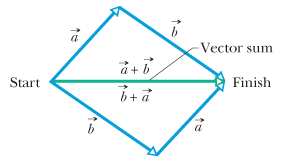
\includegraphics[scale=0.6]{commutative}
            \caption{The two vectors $\vec{a}$ and $\vec{b}$ can be added in either order (see equation \ref{eq:commutative})}
        \end{figure}

        \paragraph{Associative Law For Adding Vectors}
        \begin{equation} \label{eq:associative}
            \left( \vec{a} + \vec{b} \right) + \vec{c} = \vec{a} + \left( \vec{b} + \vec{c} \right)
        \end{equation}
        \begin{figure}[H]
            \centering
            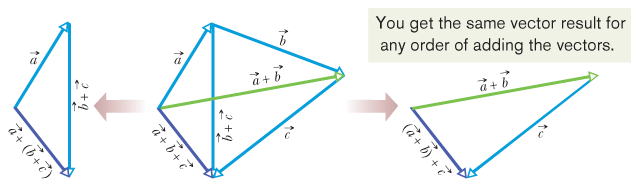
\includegraphics[scale=0.6]{associative}
            \caption{The three vectors $\vec{a}$, $\vec{b}$, and $\vec{c}$ can be grouped in any way as they are added (see equation \ref{eq:associative})}
        \end{figure}

        \paragraph{Vector Components}
        \begin{align} \label{eq:components}
            a_x = a \cos{\theta} \quad\text{and}\quad a_y = a \sin{\theta} \\
            a = \sqrt{a_x^2 + a_y^2} \quad\text{and}\quad \tan{\theta} = \frac{a_y}{a_x}
        \end{align}
        \begin{figure}[H]
            \centering
            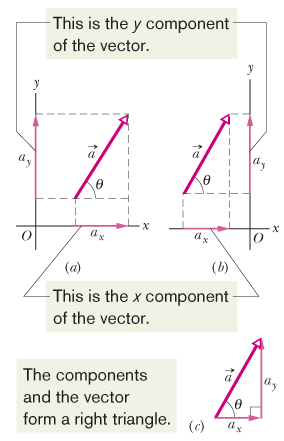
\includegraphics[scale=0.6]{components}
            \caption{The vector components $a_x$ and $a_y$ are the projections of the vector $\vec{a}$ on the $x$ and $y$ axes (see equation \ref{eq:components})}
        \end{figure}
    
    \section{Unit Vectors, Adding Vectors By Components}

        \paragraph{Unit Vectors}
        \begin{equation}
            \vec{a} = a_x \hat{\imath} + a_y \hat{\jmath} + a_z \hat{k}
        \end{equation}

        \paragraph{Adding Vectors by Components}
        \begin{equation}
            \vec{r} = \vec{a} + \vec{b} \nonumber
        \end{equation}
        \begin{equation}
            r_x = a_x + b_x
        \end{equation}
        \begin{equation}
            r_y = a_y + b_y
        \end{equation}
        \begin{equation}
            r_z = a_z + b_z
        \end{equation}

    \section{Multiplying Vectors}

        \paragraph{The Scalar/Dot Product}
        \begin{equation} \label{eq:dot-product}
            \vec{a} \cdot \vec{b} = ab \cos{\phi}
        \end{equation}
        \begin{equation}
            \vec{a} \cdot \vec{b} = a_x b_x + a_y b_y + a_z b_z
        \end{equation}
        If the angle $\phi$ between two vectors is 0\degree, the component of one vector along the other is maximum, and so is the dot product of the vectors. If, instead, $\phi$ is 90\degree, the component of one vector along the other is zero, and so it the dot product.
        \begin{figure}[H]
            \centering
            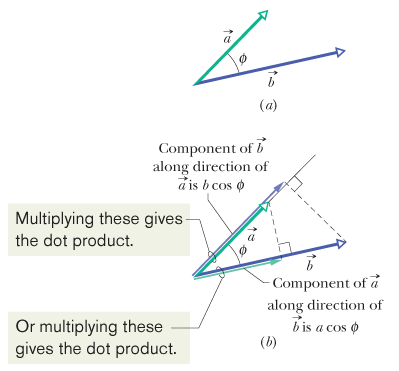
\includegraphics[scale=0.6]{dot-product}
            \caption{Two vectors $\vec{a}$ and $\vec{b}$, with an angle $\phi$ between them. Each vector has a component along the direction of the other vector (see equation \ref{eq:dot-product})}
        \end{figure}

        \paragraph{The Vector/Cross Product}
        \begin{equation}
            c = ab \sin{\phi}
        \end{equation}
        \begin{equation}
            \vec{a} \times \vec{b} =
            \begin{vmatrix}
                \hat{\imath} & \hat{\jmath} & \hat{k} \\
                a_x & a_y & a_z \\
                b_x & b_y & b_z
            \end{vmatrix}
            = \left(a_yb_z - b_ya_z\right)\hat{\imath} + \left(a_zb_x - b_za_x\right)\hat{\jmath} + \left(a_xb_y - b_xa_y\right)\hat{k}
        \end{equation}
        If $\vec{a}$ and $\vec{b}$ are parallel or antiparallel, $\vec{a} \times \vec{b} = 0$. The magnitude of $\vec{a} \times \vec{b}$, which can be written as $\\vec{a} \times \vec{b}|$, is maximum when $\vec{a}$ and $\vec{b}$ are perpendicular to each other.

\end{document}
